\chapter{Vision / perception}
\label{ch:vision}
\minitoc

Note:  This chapter is transferred from my older web site (2006), and needs some polishing.  Many links are broken.  It still represents my current view of how AGI vision should be achieved, but my focus is no longer on vision.

\section{Design philosophy}

The vision module has the following features:
\begin{enumerate}[\textbullet ]

\item \textbf{Analytical.} Visual recognition follows a reductionistic scheme in which visual objects are broken down into smaller components (3D $\rightarrow$ 2D $\rightarrow$ 1D $\rightarrow$ 0D). There is no "black-box" in this analytical scheme. 

\item \textbf{Holistic.} The intelligent agent has complete access to all visual details, down to the smallest features. However this does not mean that the system is flooded with irrelevant details � the attentional mechanism selects salient features in a scene, but the intelligent agent is free to focus attention on any minute detail. 

\item \textbf{Complete.} It has the complete range of visual functions to serve as the "eyes" of an intelligent agent. 

\item \textbf{Cognitive.} Visual recognition often involves reasoning. Therefore, the vision module interacts closely with the cognitive aspects of the intelligent agent. 
\end{enumerate}

\section{Relation between cognition and  vision}

\begin{compactenum}
	\item What Is general intelligence?
	\item The GI-vision approach
\end{compactenum}

\subsection{What is  general cognition?}

A fundamental idea of cognition is \emph{compression of information}.

Sensory experience in its raw form is like a long movie:

\begin{figure}[H]
\centering
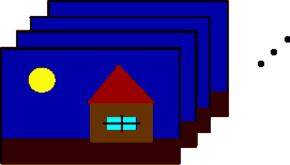
\includegraphics[scale=0.6]{Movie.png}
\end{figure}

The Visual Module compresses this movie into a semi-symbolic representation. The Cognitive Module further compresses this information. 

\begin{figure}[H]
\centering
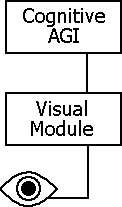
\includegraphics[scale=0.7]{GI-Vision.PNG}
\end{figure}

Compression and achieved by (statistical) \emph{pattern recognition}. For example, in the "Lena" image

\begin{figure}[H]
\centering
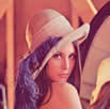
\includegraphics[scale=0.7]{Lena-Tiny.png}
\end{figure}

the object in the center can be recognized as a "face".

GI is organized hierarchically, with higher abstraction at the top. At a very high level the Lena image may be compressed symbolically as "young woman wearing a hat".

The internal representation of a GI may be a data structure containing:
\begin{compactenum}
	\item objects
	\item properties of objects
	\item relations between objects
\end{compactenum}

Some examples:
\begin{compactenum}
	\item objects: "a face", "an apple", "the letter A"
	\item properties: "face.sex = female", "apple.color = red", "letter\_A.font = Times New Roman"
	\item relations: "hat \emph{above} face", "apple \emph{on} table"
\end{compactenum}

AGI is a system that can automatically invent concepts of new objects, properties, and relations. These new concepts are in turn applied to the internal representation. For example it may learn the new property "rectangular" by looking at a lot of rectangular shapes.

\subsection{The cognitive vision approach}

Vision is basically the problem of compressing the sensory input stream in a meaningful way.

\begin{figure}[H]
\centering
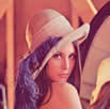
\includegraphics[scale=0.7]{Lena-Tiny.png} = "young woman wearing a hat"
\end{figure}

But there may be several \emph{levels} of representation.

As explained in the last section, each level of representation consists of:
\begin{compactenum}
	\item objects
	\item properties
	\item relations
\end{compactenum}

The pixel level is level 0 (not a representation).

 Level 1 consists of basic \emph{syntactic} features:
\begin{compactenum}
	\item edges / lines (includes straight lines and curves)
	\item regions of uniform color / intensity
	\item gradients of color / intensity
	\item textures
\end{compactenum}

These features are represented as objects. For example:
\begin{compactenum}
	\item object: curve1
	\item property: curve1.thickness = thin
	\item relation: curve1 \emph{connected-to} curve2
\end{compactenum}

At level 2 we may perform character recognition or 3D object recognition, and so on. 

The key thing here is that the vision problem is solved by  \emph{combining} GI and low-level processing. Once we have represented the image as objects + properties + relations, we can assume that a GI can handle it.

Level 1 processing is hand-programmed because it starts with pixels. Then we can rely on the GI to discover higher-level features (eg the concept "cube"). The GI will also allow us to hand-program some rules (known as \emph{knowledge insertion}), so  long periods of learning may be skipped.

\section{Machine vision --- general theory and background}

The background information on this page is adapted from [\hyperlink{ref}{Bruce, Green \& Georgeson 2003}] except otherwise stated.

\subsection{Background of general vision theories}

\subsubsection{Marr \& Nishihara (1978)}

Many people are familiar with Marr's vision theory so I won't go into details here.

This is a diagram explaining Marr's general vision framework [from \hyperlink{ref}{Herman Gomes' webpage}]:

\begin{figure}[H]
\centering
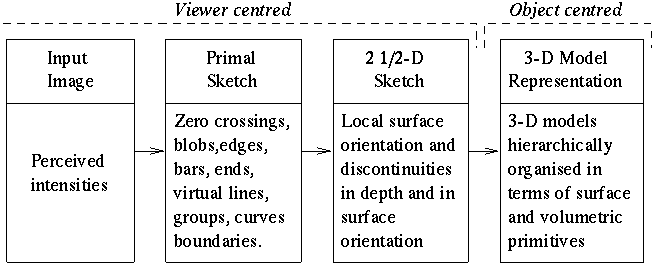
\includegraphics[scale=0.7]{MarrVisionFramework.PNG}
\end{figure}

Another famous diagram from [\hyperlink{ref}{Marr \& Nishihara 1978}] [redrawn by \hyperlink{ref}{Herman Gomes}]:

\begin{figure}[H]
\centering
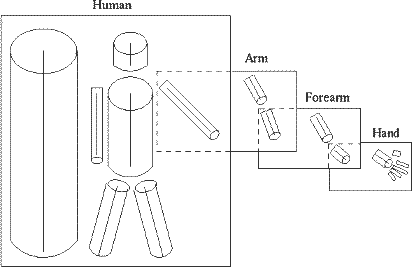
\includegraphics[scale=0.7]{Marr3DModel.PNG}
\end{figure}

 Marr \& Nishihara's theory is restricted  to describing objects using a set of \emph{generalized cones} (after [Binford 1971]).

\subsubsection{Biederman and geons}

[\hyperlink{ref}{Biederman 1987}] (web page: \href{http://geon.usc.edu/~Ebiederman/}{geon.usc.edu/\textasciitilde biederman}) proposed the "recognition by components" theory, which is closely related to Marr and Nishihara's earlier theory. In Biederman's theory, complex objects are described as spatial arrangements of basic component parts known as "geons". Geons are defined by properties that are invariant over different views. Some example geons are [taken from \hyperlink{ref}{Kirkpatrick}'s web page]:

\begin{figure}[H]
\centering
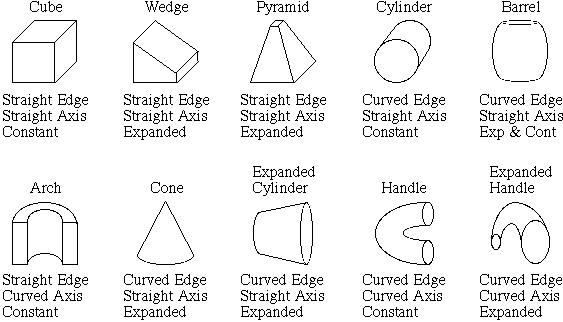
\includegraphics[scale=0.7]{geons.PNG}
\end{figure}

In particular, [\hyperlink{ref}{Biederman \& Hummel 1992}] proposed a neural network system to recognize geon-based objects:

\begin{figure}[H]
\centering
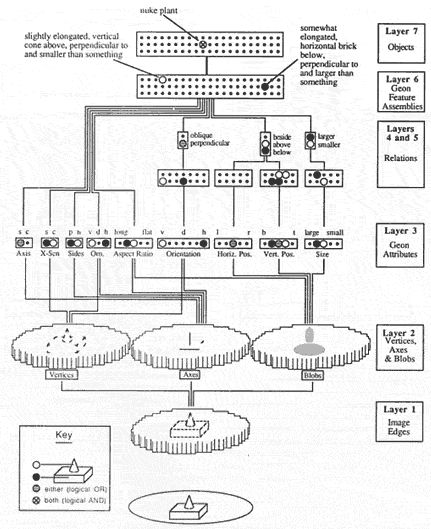
\includegraphics[scale=0.6]{BiedermanHummelNN.PNG}
\end{figure}

\subsection{Our approach}

\subsubsection{Re Marr's \& Biederman's theories}

Our approach roughly conforms to Marr's framework of  "primal sketch $\rightarrow$ 2.5D $\rightarrow$ 3D" reduction, but we describe the reduction as "0D $\rightarrow$ 1D $\rightarrow$ 2D $\rightarrow$ 3D". It may not be such a big difference, so I'll skip the discussion of this issue.

Another similarity with Marr is that I think the high-level representation is 3D in nature. But I do not restrict the representation to generalized cones only. My theory is that any 3D object can be defined by 2D surfaces, and this theory is not restricted to generalized cones or Biederman's geons.

The following examples may convince you that some shapes are not representable by common geons:

\begin{figure}[H]
\centering
%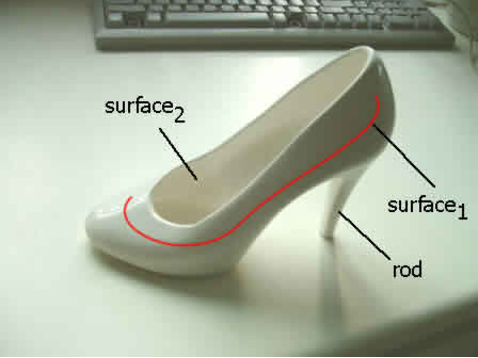
\includegraphics[scale=0.7,bb=0 0 448 336]{HighHeelAnalysis.png}
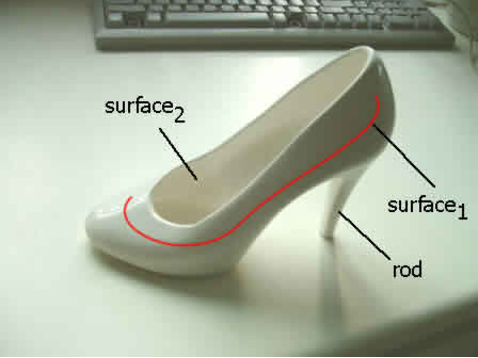
\includegraphics[scale=0.7]{HighHeelAnalysis.png}
\end{figure}

\begin{figure}[H]
\centering
%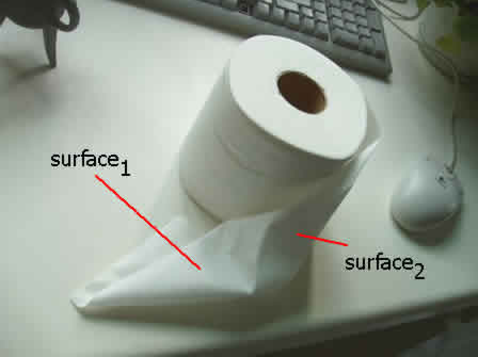
\includegraphics[scale=0.7,bb=0 0 448 336]{ToiletRollAnalysis.png}
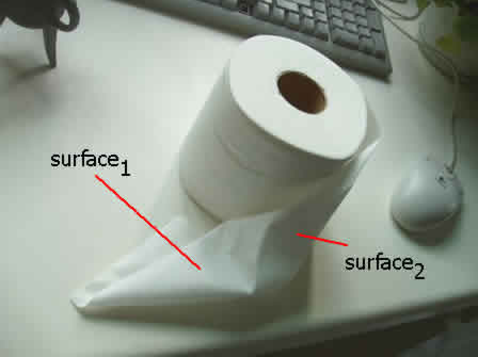
\includegraphics[scale=0.7]{ToiletRollAnalysis.png}
\end{figure}

\begin{figure}[H]
\centering
%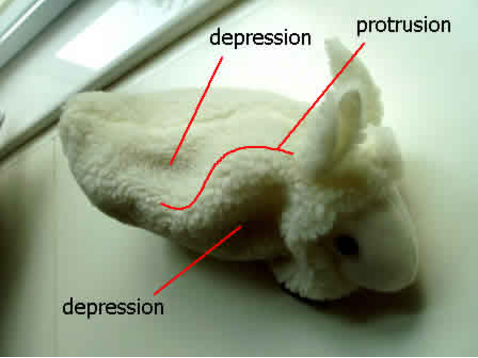
\includegraphics[scale=0.7,bb=0 0 448 336]{RabitAnalysis.png}
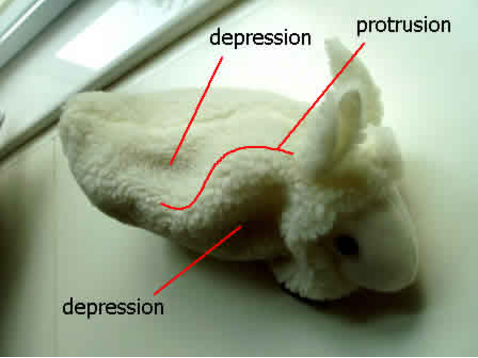
\includegraphics[scale=0.7]{RabitAnalysis.png}
\end{figure}

In all of the above cases, the objects have parts that are defined by some irregular surfaces. The geon theory may fail in such cases because Biederman et al use neural networks to learn the geons, and the geons are \emph{statistically} characterized by  vertices, blobs, and axes. This kind of learning may be slow and recognition may be erratic. What we need is a more robust theory that can represent \emph{any} 3D shape. The solution is to use \emph{logical rules} to define geons in terms of 2D lines and junctions:

\begin{figure}[H]
\centering
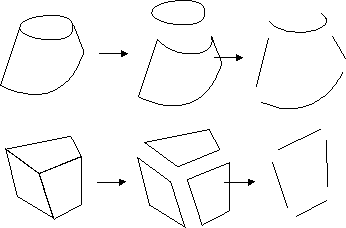
\includegraphics[scale=0.6]{PolygonDecomposition.PNG}
\end{figure}

This method is more robust and can recognize things other than common geons, such as the highheel.

\subsubsection{Shape from shading and from texture}

A number of algorithms have been developed to recover "shape from shading" with the aim of describing the 3D shape given only the pattern of reflected light intensities (for example \hyperlink{ref}{Horn \& Brooks 1989}), and "shape from texture". Shape from texture is a particularly hard problem so we will handle it later.

But  the framework of 3-2-1-0D reduction still holds for "shape-from-X". It is relatively easy to describe 3D shapes in terms of  2D surfaces, and 2D surfaces in terms of 1D contours; but it is very difficult to jump from a set of pixels straight to a 3D description. This is probably why many prior vision theories failed.

For example, to recognize the  nose, one should first recognize the shades and highlights and contours as 2D/1D features:

\begin{figure}[H]
\centering
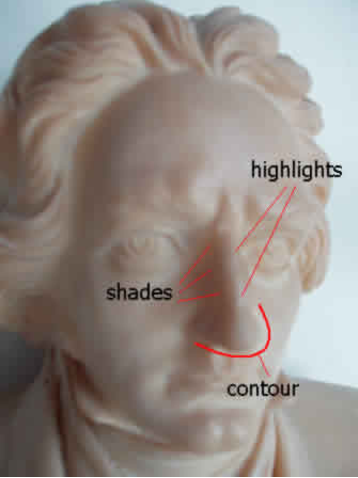
\includegraphics[scale=0.7]{BeethovenAnalysis.png}
\end{figure}

The conjunction of these 2D/1D elements allows us to recognize that the nose is a protrusion from the face, and its particular shape is jointly defined by the shapes of  2D/1D elements. It seems that a common mistake is to assume that the brain immediately recognizes the nose as a 3D shape  from pixel-level data, without going through the intermediate stages, because the brain is usually unconscious of those intermediate stages.

Recognizing shading as 2D features will require special algorithms (so does recognizing textures). At first we will focus on using exclusively edge detection (contours) to recognize objects.

\subsubsection{References}

[Biederman 1987] \emph{Recognition by components: A theory of human image understanding}. Psychological Review, 94, 115-145

[Biederman \& Hummel 1992] \emph{Dynamic binding in a neural network for shape recognition}. Psychological Review 99, 480-517 

[Binford 1971] \emph{Visual perception by computer}. Paper presented at the IEEE Conference on Systems and Control, December 1971, Miami

[Bruce, Green \& Georgeson 2003] \emph{Visual Perception --- Physiology, Psychology and Ecology}, Psychology Press, NY

[Gomes 2000] Herman Gomes' web page: \emph{Marr's Theory: From primal sketch to 3-D models}, \href{http://homepages.inf.ed.ac.uk/rbf/CVonline/LOCAL_COPIES/GOMES1/marr.html}{http://homepages.inf.ed.ac.uk/rbf/CVonline/LOCAL\_COPIES/GOMES1/marr.html}

[Horn \& Brooks 1989] \emph{Shape from shading}. MIT Press, Cambridge, MA

[Kirkpatrick K] Web page on object recognition \href{http://www.pigeon.psy.tufts.edu/avc/print/kirkpatrick/kirkpatrick_figprint.htm}{http://www.pigeon.psy.tufts.edu/avc/print/kirkpatrick/kirkpatrick\_figprint.htm}

[Marr \& Nishihara 1978] \emph{Representation and recognition of the spatial organization of 3D shapes}. Proceeding of the Royal Society of London, series B, 200, 269-294 

\section{Requirements of general vision}

\underconst

\section{Basic vision scheme}

Our approach to solving the general vision problem is to combine vision with GI (general intelligence). See \href{Vis-Cognition.htm}{an introduction to GI-vision}.

The basic tenets of my vision theory are:
\begin{compactenum}
	\item  Break down the image via 3D-2D-1D-0D primitives
	\item  Apply  machine learning to represent the image symbolically
\end{compactenum}

I have thought about the vision problem for 1-2 years and studied many real images to conclude that "everything under the sun" can be recognized by this method. A  paper will be published to explain the theory in detail.
\underconst
\begin{compactenum}
	\item \hyperlink{3210DReduction}{3-2-1-0D reduction}
	\item \hyperlink{LogicalRepresentation}{Logical representation}
	\item \hyperlink{MachineLearning}{Machine learning}
	\item \hyperlink{Example}{Example: quadrilateral}
	\item \hyperlink{ApproximateRecognition}{Approximate recognition and feedback}
	\item \hyperlink{Attention}{Searchlight attention}
	\item \hyperlink{Relations}{Relations between objects}
	\item \hyperlink{Architecture}{Architecture of the vision module}
\end{compactenum}

\subsection{3-2-1-0D reduction}

The premise is that any 3D object (or its "geon-like" components) can be defined by  2D surfaces, which are in turn defined by 1D lines. Please refer to \href{Vis-Background.htm}{General vision theory and background} for the justification of this point.

\begin{figure}[H]
\centering
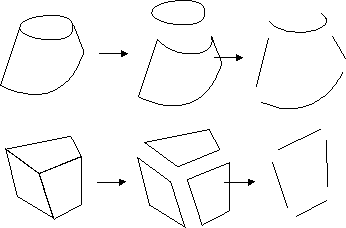
\includegraphics[scale=0.6]{PolygonDecomposition.PNG}
\end{figure}

The image is first broken down into 0D/1D primitives (such as edgels and lines). Then 2D elements are recognized (such as regions and surfaces). Then 3D objects are recognized (blocks, 3D geons, etc).

The decompositions are represented by graphical data structures (ie nodes and links). Nodes are primitive elements; Links represent the spatial relations between them.

Details of \href{Vis-3210D-Reduction.htm}{3-2-1-0D reduction}.

Our 1D-2D levels may coincide with David Marr's primal sketch level. Here we reframe these levels under the \href{Vis-PrimalSketch.htm}{primal sketch} framework.

\subsection{Logical representation}

The first step is to transform the image to a logical representation:

\begin{figure}[H]
\centering
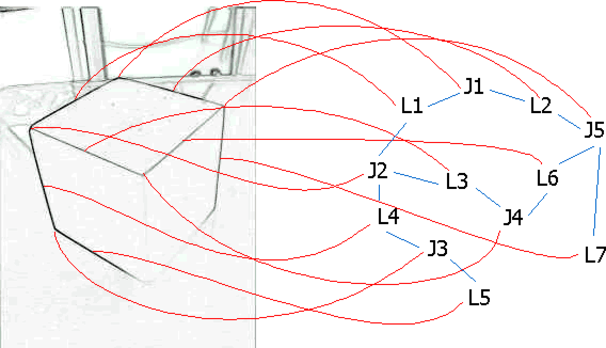
\includegraphics[scale=0.8]{VisioLogicalTransform.png}
\end{figure}

On the left hand side is the image; we have applied  Sobel edge detection. On the right hand side is the logical representation. L1,L2,L3... = lines, J1,J2,J3... = junctions. The blue lines represent how the elements are connected. Other details at the background have not been represented.

For simple, uncluttered scenes, this scheme will work fine. The idea is that every detail, no matter how irregular, would be represented using this logical representation (using elements such as blobs and shades in addition to lines, junctions, etc).

This approach requires a lot of patience, but ultimately we would be able to analyse everything in the world. Other approaches such as neural network or SIFT are not as general or comprehensive.

We may use neural networks at the lowest level for recognizing "edgels". Then the next stage is to join the edgels to recognize longer lines.

\subsection{Machine learning}

What we need is a special kind of machine learning known as inductive learning (as opposed to deductive learning). In inductive learning a system tries to induce \emph{general rules} from a set of observed instances ("learning by examples").

There should be an underlying knowledge representation (KR) or  "calculus" that encompasses what kinds of rules are possible. The most common KR scheme is first-order predicate logic, often abbreviated as FOL (first order logic). Other options include: neural networks, semantic networks, conceptual graphs, Bayesian networks, etc.

It is not easy to determine what kind of KR is adequate for our task at hand (visual recognition). Therefore we start with something simple and similar to FOL and see if it needs to be expanded or modified.

Details of \href{Vis-InductiveLearning.htm}{inductive learning}. 

\subsection{Example: quadrilateral}

Any figure with 4 sides (straight lines).

Define the predicate \texttt{Terminates(edge,vertex)}  to indicate when an edge terminates with a vertex.

\begin{figure}[H]
\centering
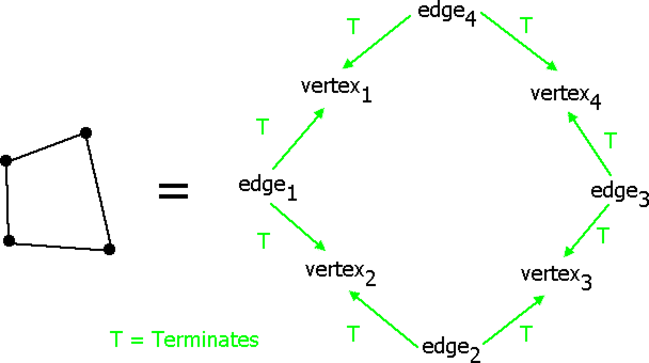
\includegraphics[scale=0.6]{Quadrilateral.png}
\end{figure}

This results in the set of logical statements:
\begin{quote}

\texttt{Terminates(edge$_1$,vertex$_1$) = true
\\
    Terminates(edge$_1$,vertex$_2$) = true
\\
    Terminates(edge$_2$,vertex$_2$) = true 
\\
    Terminates(edge$_2$,vertex$_3$) = true 
\\
    Terminates(edge$_3$,vertex$_3$) = true
\\
    Terminates(edge$_3$,vertex$_4$) = true 
\\
    Terminates(edge$_4$,vertex$_4$) = true 
\\
    Terminates(edge$_4$,vertex$_1$) = true
  }
\end{quote}

Perhaps, we can introduce a new predicate \texttt{Connects(edge,vertex$_1$,vertex$_2$)} to simplify the above to:
\begin{quote}

\texttt{Connects(edge$_1$,vertex$_1$,vertex$_2$) = true
\\
    Connects(edge$_2$,vertex$_2$,vertex$_3$) = true
\\
    Connects(edge$_3$,vertex$_3$,vertex$_4$) = true
\\
    Connects(edge$_4$,vertex$_4$,vertex$_1$) = true}
\end{quote}

Assuming that the "universe"  is a connected graph that the system is currently paying attention to, now we can easily define the 0-ary predicate \texttt{Quadrilateral()} using \emph{typed logic}:
\begin{quote}

\texttt{Quadrilateral() :-}
\begin{quote}

\texttt{$\exists $ e$_1$:edge
\\
      $\exists $ e$_2$:edge
\\
      $\exists $ e$_3$:edge
\\
      $\exists $ e$_4$:edge
\\
      $\exists $ v$_1$:vertex
\\
      $\exists $ v$_2$:vertex
\\
      $\exists $ v$_3$:vertex
\\
      $\exists $ v$_4$:vertex
\\
      Connects(e$_1$,v$_1$,v$_2$) $\wedge$
\\
      Connects(e$_2$,v$_2$,v$_3$) $\wedge$
\\
      Connects(e$_3$,v$_3$,v$_4$) $\wedge$
\\
    Connects(e$_4$,v$_4$,v$_1$)}
\end{quote}
\end{quote}

This is just an example. Please refer to this page concerning  various issues of \href{Vis-InductiveLearning.htm}{inductive learning}. Some other issues specific to vision are discussed as follows.

\subsection{Approximate recognition and feedback}

One problem is that primitive features  are often fuzzy and should be approximately recognized.

For example, in the image below, 2 edges and 1 vertex are almost invisible, yet given the current \emph{context} they should be interpreted as edges and vertex. The context is important because very weak features would be regarded as noise otherwise:

\begin{figure}[H]
\centering
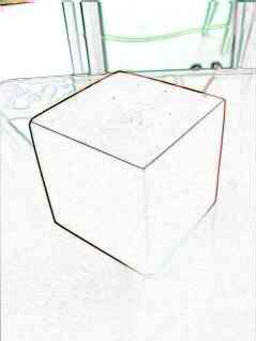
\includegraphics[scale=0.8]{CubeMissingEdge.png}
\end{figure}

The feedback mechanism should work this way: When the Recognizer finds that a concept is "almost" recognized (eg with the majority of conjuncts being true), it will select the remaining features that are not yet matched and send them to the lower-level Recognizer, which would then lower its \emph{threshold} for recognizing those features.

This requires 2 things:
\begin{compactenum}
	\item The Recognizer  should measure a \emph{degree of certainty} associated with each feature being recognized.
	\item  The Recognizer  at the lower level should be able to use an feedback cue to look for certain features. This may require performing an "inversion" of the cue.
\end{compactenum}

A detailed explanation of the feedback mechanism will be presented soon.
\underconst

\subsection{Searchlight attention}

Another problem is that real world images are often composed of many cluttered elements, so we need to use a "searchlight" to look for individual objects in a cluttered scene.

Searchlight attention is closely related to the feedback mechanism outlined above. Due to limited computational resources we can only extract features within a "fovea" of attention. If a concept is detected to be "almost" complete, the searchlight will direct the fovea to focus on  areas that are likely to complete the concept, with a concomitant decrease of attention to other areas.

This requires the searchlight to know \emph{where} to search for the feedback cue. In a sense this also requires inversion of the cue.

\subsection{Relations between objects}

The vision system not only has to recognize individual objects, but also relations among them (represented as links).

The way to achieve this is to pay attention to individual objects \emph{sequentially}. Relations are then recognized by the identities of the objects in the sequence and by how the searchlight moved.

In our logical formulation, an object is recognized by a 0-ary predicate such as \texttt{Cube$_1$()}. Then we have to bring this object to the \emph{next} level of recognition, where it is represented by a variable such as \texttt{cube$_1$}. Only then we would be allowed to denote a relation like \texttt{Above(cube$_1$,cube$_2$)} at this level.

Recognition at each level is \emph{independent} of recognition at other levels, except for the feedback mechanism.

The "main loop" of the Recognizer would be using the searchlight to scan around the image, and recognizing individual objects. When the searchlight moves, its movement will be recorded and later used to form the link between the current object and the next object.

\subsection{Architecture of the vision module}

\begin{figure}[H]
\centering
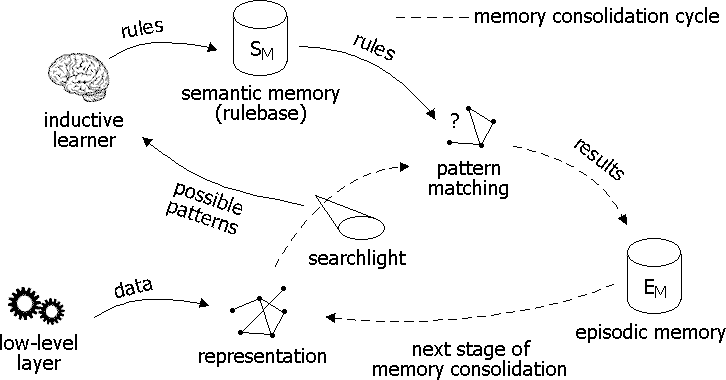
\includegraphics[scale=0.6]{VisionArchitecture.PNG}
\end{figure}

The operation of the above module is typical of a rule-based system, except that there is a "loop" in the lower right corner that repeats the pattern matching process at multiple levels. What this means is that the raw sensory experience goes through multiple stages of memory consolidation via pattern matching. For details please refer to \href{GI-MemorySystems.htm}{Memory systems}. 

This architecture has to be integrated with the larger GI (general intelligence) framework, to form a complete intelligent agent. Please refer to \href{GI-architecture.htm}{GI architecture}.

\section{Details of  3-2-1-0D reduction}

An illustrated example ("cube") is \href{Vis-Example.htm}{here} (incomplete)
 
\underconst

The following is a very tentative outline, the order of steps may be wrong and additional steps may be needed...

\subsection{Stage 1: 1D Analysis }

1. Edge detection --- distinguish between single-pixel lines and thick lines.

2. \href{Vis-1DTaxonomy.htm}{Classification of 1D lines}: straight lines, curves, junctions. From this point on the representation is a collection of discrete lines and junctions: qualitative / structural rather than quantitative / spatial / continuous.

3. Good continuation --- line / curve completion.

\begin{figure}[H]
\centering
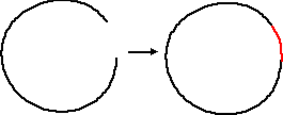
\includegraphics[scale=0.6]{GoodContinuation.png}
\end{figure}

4. Contour simplification --- the image is represented by both simple and detailed contours (allowing redundency in representation).

\begin{figure}[H]
\centering
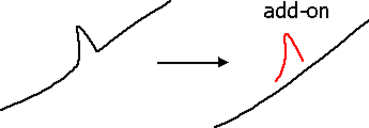
\includegraphics[scale=0.6]{ContourSimplification.png}
\end{figure}

Some things can be recognized at this stage: text, handwriting, 1D graphics.

\subsection{Stage 2: 2D Analysis}

5. Characterization of regions according to color, shading or textures (segmentation).

6. Classification of 2D shapes

\underconst

7. Extract gestalt-induced contours --- (a) numerous small, identical / similar elements may induce contours; (b) the absence of features induces "invisible" contours

\begin{figure}[H]
\centering
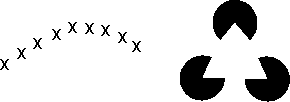
\includegraphics[scale=0.6]{GestaltContours.PNG}
\end{figure}

8. Deal with occlusion.

Some 2D graphics may be recognized at this stage.

\subsection{Stage 3: 3D Analysis}

9. \href{Vis-3DTaxonomy.htm}{Classification of 3D lines / surfaces}.

10. Identify objects according to templates or algorithms. The question is how to define an object such as the object classes "bottle", "books", "faces", etc.

\section{Primal sketch project}

\subsection{Background}

According to Marr, the primal sketch represents changes in light intensity occuring over space in the image. It also organises these local descriptions of intensity change into a 2D representation of image regions and the boundaries between them.

Specifically, the primal sketch may include elements such as edges (curves or straight lines), color blobs, ends, junctions (of edges), texons, etc.

Marr's vision scheme consists of 3 levels:
\begin{compactenum}
	\item primal sketch
	\item 2.5D
	\item 3D
\end{compactenum}

My \href{Vis-BasicScheme.htm}{vision scheme} is slightly different which goes from 3D, 2D to 1D. This difference may not be all that important; what is important is how best to recognize features at various levels, from a computational viewpoint. The primal sketch is an essential stage of any complete vision system.

What I propose is that the output of the primal sketch should be represented as a symbolic web with links that are logical predicates. Developing such a low-level layer would make a tremendous contribution towards computer vision.

\subsection{What we're trying to do }

\subsubsection{1. Obtaining the primal sketch }

One solution to the primal sketch problem (I have not surveyed the topic completely) is presented in [\hyperlink{Ref}{Gao, Zhu \& Wu 2006}], "Primal Sketch: Integrating Texture and Structure" (\href{http://www.stat.ucla.edu/~sczhu/papers/primal_sketch.pdf}{pdf}), by researchers in the UCLA Center for Image and Vision Science.

As explained in the paper, an input image is separated into 2 regimes, one "sketchable" and the other "non-sketchable". The sketchable regime is one of low entropy where the image can be represented by a sparse-coding sum of primitive features; the non-sketchable regime is of relatively higher entropy where sparse-coding is no longer practical and those areas of the image should be represented as \emph{textures}.

In our project we were trying to deal with the type of low level feature extraction in the sketchable regime, while temporarily ignoring textures. I'm currently trying to have a collaboration with the UCLA group or possibly license their technology.

\subsubsection{2. Output an attributed graph}

After obtaining the primal sketch, the second task is to represent the image as an attributed graph. This has been partly accomplished in [\hyperlink{Ref}{Han \& Zhu 2005}], \emph{Bottom-up/Top-down Parsing with Attributed Graph Grammar} (\href{http://www.stat.ucla.edu/~sczhu/papers/PAMI_Grammar_rectangle.pdf}{pdf}), for some simple shapes.

The goal of our project is to output attributed graphs similar to the above kind for all sorts of images. The expressiveness of the attributed graph may be comparable to that of first-order predicate logic.

 Then the next step is to delegate the tasks of recognition and inference to an intelligent agent or cognitive architecture.

\subsubsection{3. Handover to intelligent agent}

The following tasks may be handled by the intelligent agent:
\begin{compactenum}
	\item pattern recognition
	\item attentional mechanism (eg focusing attention to various features or objects)
	\item learning of concepts and facts (declarative and episodic memory)
	\item complex inference (for example, a chair is "anything that can be sat on", may involve procedural memory)
\end{compactenum}

The division of labor can avoid repeating these tasks for vision and for general cognition.

Currently we are considering the following intelligent agents for integration with vision:
\begin{compactenum}
	\item Novamente (has an architecture integrating perception and cognition)
	\item Soar (has provisions for sensory perception)
	\item Cyc (depends on its proprietary inference engine)
	\item ACT-R
	\item EPIC
	\item IDA (intelligent distribution agent, Stan Franklin)
\end{compactenum}

Basically any general cognitive architecture that can handle sensory perception, can use our vision module.

\subsubsection{References}

[Guo,  Zhu \& Wu 2006] \emph{Primal Sketch: Integrating Texture and Structure}, 
Computer Vision and Image Understanding, 2006 (Accepted for the Special Issue on Generative Model Based Vision) (\href{http://www.stat.ucla.edu/~sczhu/papers/primal_sketch.pdf}{pdf})

[Han \& Zhu 2005] \emph{Bottom-up/Top-down Image Parsing with Attribute Graph Grammar}, 
Statistical preprint, 2005. Submitted to PAMI (\href{http://www.stat.ucla.edu/~sczhu/papers/PAMI_Grammar_rectangle.pdf}{pdf}) 

\section{Classification of 1D Shapes}

Here I attempt to classify all 1D shapes (contours) into primitive elements (lines, curves, junctions).

My view is that the vision problem (especially the recognition of 3D objects) can be solved via a 3D $\rightarrow$ 2D  $\rightarrow$ 1D process. All  3D objects can be defined by 2D elements (surfaces), and all 2D shapes (areas) can be defined by 1D contours.

\subsection{Main Classes}

All 1D shapes can be decomposed into: 

\begin{figure}[H]
\centering
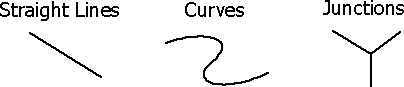
\includegraphics[scale=0.7]{1DClasses.PNG}
\end{figure}

\textbf{Properties:} (thickness, color, texture)

\subsection{1. Straight Lines}

\textbf{Properties:} (position, length, orientation, end points)

\subsection{2. Curves}

4 subtypes:

\subsubsection{1. Simple Curves}

Curves with no inflections:

\begin{figure}[H]
\centering

\includegraphics[scale=0.7]{CurvesClasses.PNG}
\end{figure}

\textbf{Properties:} (position, length, orientation, end points, curvature)

\subsubsection{2. Ellipses/Circles}

\begin{figure}[H]
\centering

\includegraphics[scale=0.7]{EllipsesClasses.PNG}
\end{figure}

\textbf{Properties:} (position, orientation, size, axes ratio)

\subsubsection{3. Complex Curves}

\begin{figure}[H]
\centering
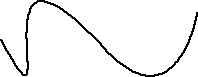
\includegraphics[scale=0.7]{ComplexCurves.PNG}
\end{figure}

\textbf{Properties:} (position, length, end points, \# of inflections, curvatures) 

\subsubsection{4. Complex Loops}

\begin{figure}[H]
\centering
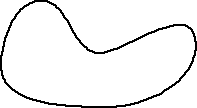
\includegraphics[scale=0.75]{ComplexLoops.PNG}
\end{figure}

\textbf{Properties:} (position, area, shape description, \# of inflections)

\subsection{3. Junctions}

\textbf{Properties:} (position, \# of lines, angles) 

3 subtypes:

\subsubsection{1. L}

\begin{figure}[H]
\centering
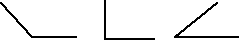
\includegraphics[scale=0.7]{Junctions-L.PNG}
\end{figure}

\subsubsection{2. T}

\begin{figure}[H]
\centering
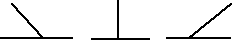
\includegraphics[scale=0.7]{Junctions-T.PNG}
\end{figure}

\subsubsection{3. Y }

\begin{figure}[H]
\centering
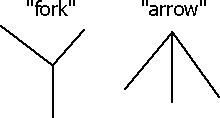
\includegraphics[scale=0.7]{Junctions-Y.PNG}
\end{figure}

\subsubsection{4. X}

\begin{figure}[H]
\centering
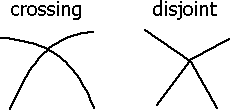
\includegraphics[scale=0.7]{Junctions-X.PNG}
\end{figure}

May have $>$4 lines of convergence.

\subsection{Examples}

The following examples illustrate the concept of \textbf{self-aggregation}, which means edgel detectors (or "neurons") aggregating with others with similar attributes such as color, orientation, etc.

A line with a slight bend: (the bending is noticed even though it is very slight, because the A \& B parts are very straight in contrast):

\begin{figure}[H]
\centering
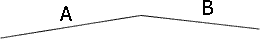
\includegraphics[scale=0.7]{Line1.PNG}
\end{figure}

This line has many bends but is still recognized as a continuous line: 

\begin{figure}[H]
\centering
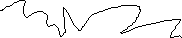
\includegraphics[scale=0.7]{Line2.PNG}
\end{figure}

For the following line, a simple algorithm may classify it as a curve, but people will describe it as: two slightly curved lines A \& C, bending at a point B. This illustrates the context-dependent aspect of human vision.

\begin{figure}[H]
\centering
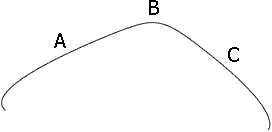
\includegraphics[scale=0.7]{Line3.PNG}
\end{figure}

The following is yet another context-dependent example: we see 2 "shaky" but straight lines bending at an angle.

\begin{figure}[H]
\centering
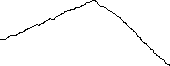
\includegraphics[scale=0.7]{Line4.PNG}
\end{figure}

What is a "straight" line is relative: B is straighter than A but in the above context A is also considered a straight line. 

\begin{figure}[H]
\centering

\includegraphics[scale=0.7]{Line7.PNG}
\end{figure}

People will describe the following as a regular "sine" curve:

\begin{figure}[H]
\centering

\includegraphics[scale=0.7]{Line5.PNG}
\end{figure}

This is also a simple curve that people can describe with basic features such as crest and trough and being smooth:

\begin{figure}[H]
\centering
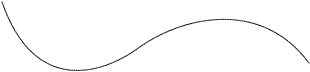
\includegraphics[scale=0.7]{Line6.PNG}
\end{figure}

People can also characterize line junctions with special attributes, eg a "smooth" junction:

\begin{figure}[H]
\centering
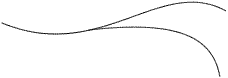
\includegraphics[scale=0.7]{Line8.PNG}
\end{figure}

This can be considered as  1 line with 2 colors:

\begin{figure}[H]
\centering

\includegraphics[scale=0.7]{Line9.png}
\end{figure}

This is also considered a simple curve with internal texture:

\begin{figure}[H]
\centering

\includegraphics[scale=0.7]{Line10.PNG}
\end{figure}

\underconst

\section{Classification of 2D features}

\underconst

\section{Classification of 3D Shapes}

There are a limited number of possible 3D contours and junctions. The technique of labeling all contours and junctions consistently is known as \emph{relaxation labeling} and has grown into a large area of work.

We should work out the rules of arbitrary 3D object construction...

\underconst

\subsection{3D Edges}

\begin{figure}[H]
\centering
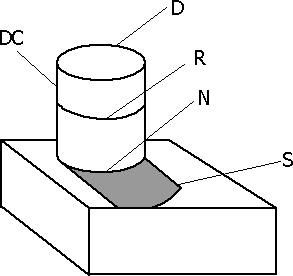
\includegraphics[scale=0.7]{3DContours.PNG}
\end{figure}

D = discontinuity of distance of object, discontinuity of normal of object surface

DC = discontinuity of distance of object, continuous normal of object surface

N = discontinuity of normal of object surface 

R = change of reflectance

S = shadow

Each type of contour has its characteristics such as shading. Such characteristics help to infer its type.

\subsection{3D Junctions }

There are 16 topologically possible line junctions in the "trihedral blocks world":

\begin{figure}[H]
\centering
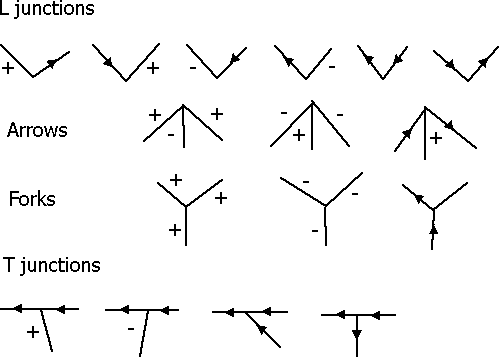
\includegraphics[scale=0.7]{16Junctions.PNG}
\end{figure}

+ and - indicates whether a crease is convex or concave, respectively. An arrow indicates a "blade" formed by a discontinuity of distance (same as the D-type contour above). The direction of the arrow indicates which side is the \emph{occluding} surface, which by convention is to the right.

We should extend this analysis to arbitrary 3D shapes.

\section{Inductive learning for vision}

Inductive logic programming seems to be the harder part of our project (in fact ILP is considered one of the hardest areas in computer science!)

\subsection{Background to ILP (inductive logic programming)}

\subsubsection{Books and internet resources}
\begin{compactenum}
	\item \emph{Machine Learning} [Mitchell 1997] \emph{}has a chapter on "Learning Sets of Rules" which is a good introduction.
	\item \emph{AI: A Modern Approach} talks about ILP in chapter 19
	\item {\normalsize This 1994 book by N. Lavrac and S. Dzeroski is free for download: \textit{\href{http://www-ai.ijs.si/SasoDzeroski/ILPBook/}{Inductive Logic Programming: Techniques and Applications}.}}
	\item Stephen H Muggleton's website on ILP: \href{http://www.doc.ic.ac.uk/~shm/}{www.doc.ic.ac.uk/\textasciitilde shm/}
	\item Peter A Flach's website: \href{http://www.cs.bris.ac.uk/~flach/}{www.cs.bris.ac.uk/\textasciitilde flach} and his PowerPoint on \href{http://macflach.cs.bris.ac.uk/~flach/presentations/CL2000HTML/CL2000.ppt}{Knowledge Representation and ILP}.
	\item many more...
\end{compactenum}

\subsubsection{A simple ILP example}

To learn the relation \texttt{Daughter(x,y)}.

A database may have the following facts:
\begin{quote}

\texttt{Male(mary) = false
\\
    Female(mary) = true
\\
    Mother(mary, louise) = true
\\
    Father(mary, bob) = true
\\
    Daughter(bob, mary) = true
\\}etc......
\end{quote}

After presenting a large number of such facts,this rule may be learned:
\begin{quote}

\texttt{IF Father(y,x) $\wedge$ Female(y) THEN Daughter(x,y)}
\end{quote}

\subsubsection{Existing ILP software}
\begin{compactenum}
	\item FOIL
	\item  CIGOL ('logic' spelt backwards)
	\item GOLEM
	\item  PROGOL
	\item LINUS
	\item etc...
\end{compactenum}

\subsection{Special concerns related to vision}

The "fovea" focuses on a particular area or scale of an image. Low-level feature extraction results in a graphical representation of the scene. The nodes and links of this graphical representation is then converted to a set of logical statements. This set is then taken to be the "model" (possible world) of the logic.

Low-level feature extraction has to use the searchlight mechanism to discover the spatial relations among features, and then outputs a graphical / logical representation for the next level. The "universe" of the logic at each level is distinct from each other.

\subsection{Why use logic?}

 Our scheme is to reduce 3D to 2D to 1D to 0D. Along this route, many concepts need to be defined:
\begin{compactenum}
	\item  First, we have the image decomposed into edgels, which are the lowest-level features.
	\item  Then we define "lines" and "curves" as collections of contiguous edgels.
\\
    (From 0D to 1D: line = conjunction of edgels)
	\item  Then we define "polygons", "parallelograms", "squares", etc as collections of lines.
\\
    (From 1D to 2D: surface = conjunction of lines) 
	\item  Then we can define "cylinders", "blocks", etc as collection of surfaces.
\\
    (From 2D to 3D: volume = conjunction of surfaces)
	\item Then we define objects such as "bicycles", "wheels", etc as composed of primitive geons.
\end{compactenum}

If we can enter all these things as rules in a knowledgebase, we have a vision system that operates by the rules. Our strategy is to encode these rules as \emph{logical formulas}.

\subsubsection{Why not neural networks? }

The use of logic to represent rules (definitions) has a tremendous advantage over neural networks. For example, a quadrilateral is defined as any figure with 4 sides. Quadrilaterals can appear in all sizes and shapes, yet we have no problem recognizing any of them. With predicate logic, we can easily define a quadrilateral in terms of edges and vertices (an example is given in \href{Vis-BasicScheme.htm}{Vision scheme}). The resulting formula is very succinct and is capable of covering all possible cases (ie it has low algorithmic complexity).

On the other hand, in neural networks we have to learn the concept of quadrilaterals in a high dimensional space populated with many instances of quadrilaterals. Such a \emph{statistical} learning method continually "molds" the classification space into the right shape, with incremental steps, which is extremely inefficient and prone to errors. In other words, it fails to reduce algorithmic complexity significantly.

The essense of logic is that it can represent \emph{objects} and their \emph{relations}. Objects are variables and relations are predicates. The use of variables allows logic to represent many things \emph{succinctly}. For example I can use the predicate \texttt{Kicks(x,y)} to mean x kicks y. The predicate can be used to denote "boy kicks ball", "girl kicks dog", or "John kicks Mary" even though these events are very dissimilar. Thus the great expressiveness of predicate logic. Most artificial neural networks nowadays cannot express things with variables.

You may argue that the brain is a neural network and so they must be capable of achieving vision and cognition. I guess the answer is that the brain probably uses neurons to perform some sort of symbolic/logical computations, rather than statistical learning as many neuroscientists now assume. Unfortunately how the cortex performs computation is still a \emph{terra incognita}.

\subsection{What's the use of inductive learning?}

For a very simple vision system, inductive learning is not needed. All we need is to  patiently enter  definitions of shapes / objects into a logical knowledgebase. Then the system can recognize those things. 

Inductive learning is needed for 2 purposes:
\begin{compactenum}
	\item  teaching by "show and tell";
	\item  automatically discovering useful concepts.
\end{compactenum}

\subsubsection{"Show and tell"}

It is far easier to show the computer a number of examples of an object (eg "pineapple") than to explicitly define the general appearance of that object. The inductive learner will automatically generalize from the exemplars.

\begin{figure}[H]
\centering
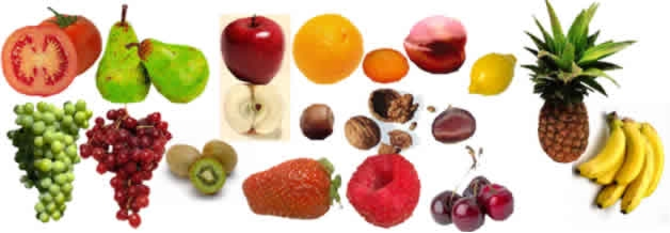
\includegraphics[scale=0.7]{Fruits.png}
\end{figure}

\subsubsection{Automatic discovery of useful concepts}

This is an advanced topic, but of great practical value. A "useful" concept is one that helps meaningfully to characterize a broad class of objects. For example the concept of "leaf" may characterize the leaves often attached to many types of fruits, and may also apply to flowers and trees. So it is a useful concept.

Another useful concept is "parallelogram" which often occurs in the views of rectangular blocks. If we do not use the concept of parallelogram then the description of rectangular blocks may become cumbersome.

 In other words, a useful concept reduces description lengths. But if we are talking about the total description length of a knowledgebase, then the discovery of "good" concepts requires global searching. This is therefore a computational hard problem. 

\subsection{Inductive learning methods}

\underconst

We are currently looking for researchers in ILP to collaborate with us to develop the Inductive Learner...

\subsection{Outstanding questions}

Do we need some special inference operations outside of predicate logic? Such as stochastic logic?

When doing higher-level recognition, does the Recognizer need to be aware of the constituents of high-level features? Eg, that a line is a collection of edgels?

\section{Depth / distance estimation}

\underconst

\section{Motion and event detection}

\underconst

\section{Texture}

\underconst

\section{Stereopsis}

\underconst

\section{Sample images}

Sample images are currently hosted at:\\
\hspace*{1cm} http://www.geocities.com/genericai/Vis-SampleImages.htm
but the site will soon be closed (around October 2009).  I will try to relocate them somewhere.
